\documentclass{article}
\usepackage{graphicx}
\usepackage{amsmath}
\usepackage{pgfplots}
\usepackage{physics}
\usepackage{cancel}
\usepackage{enumitem}
\usepackage{txfonts}

\pgfplotsset{compat=1.18}

\pgfplotsset{compat=1.18}

\usepackage[a4paper, top=1cm, bottom=2cm, left=2cm, right=2cm, includehead, includefoot]{geometry}

\begin{document}

\noindent
Physics 4B - Electromagnetism \hfill Prof. Alfred Cauthen

\noindent\rule{\textwidth}{0.4pt}

\begin{center}
    \textbf{\LARGE Homework 1} \\
    \vspace{12pt}
    \large Aaron W. Tarajos \\
    \textit{\today}
\end{center}

\noindent\rule{\textwidth}{0.4pt}

\section*{21-3 Question 2}
Figure 21-12 shows three pairs of identical spheres that are to be touched together and then separated. 
The initial charges on them are indicated. 
Rank the pairs according to (a) the magnitude of the charge transferred during touching and (b) the charge left on the positively charged sphere, greatest first.

\begin{figure}[ht]
    \centering
    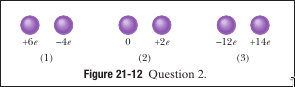
\includegraphics[scale=0.75]{image.png}
\end{figure}

\subsection*{Solution}
\textbf{Part a:} The first pair transfers $4e$, the second pair transfers $0e$ of chrage, and the third pair transfers $12e$ of charge.

\[
    \boxed{\text{pair 3}  > \text{pair 1} > \text{pair 2}}
\]
\textbf{Part b:} The positively charged sphere is left with $2e$ in all three transfers.

\section*{21-3 Question 8}
Figure 21-17 shows four arrangements of charged particles.
Rank the arrangements according to the magnitude of the net electrostatic force on the particle with charge +Q, greatest first.

\begin{figure}[ht]
    \centering
    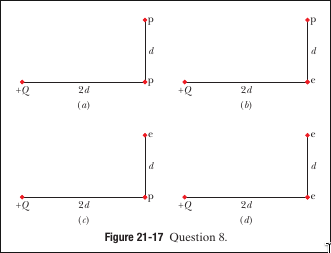
\includegraphics[scale=0.75]{image-2.png}
\end{figure}

\subsection*{Solution}
The forces magnitude in $(a)$ and $(d)$ are the same because the configuration of the system is the same just with the opposite charge which changes the direction of the force not the magnitude.
The same can be said for the relationship between $(b)$ and $(c)$, although their magnitude is less than the other configuration because the difference in charge of the particles acting on $Q$ create forces of the opposite sign in one direction which reduces the magnitude of the total force.
Therefore we have; 

\[
    \boxed{a = d > b = c}
\]

\section*{21-3 Question 10}
In Fig.21-19, a central particle of charge $-2q$ is surrounded by a square array of charged particles, separated by either distance $d$ or $d/2$ along the perimeter of the square.
What are the magnitude and direction of the net electrostatic force on the central particle due to the other particles?

\begin{figure}[ht]
    \centering
    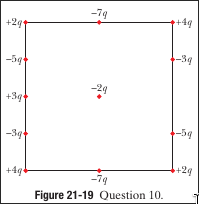
\includegraphics[scale=0.75]{image-3.png}
\end{figure}

\subsection*{Solution}
Notice that every single charge has a charge on of equal magnitude exactly opposite to it in the system with exception of the $+3q$ charge to the left of the central particle.
Therefore the net force in every other direction will sum to zero with the exception of that one where we have;

\[
    F_e = k \frac{|3||-2|}{d^2/2^2} = \boxed{k \frac{24}{d^2} \quad \text{to the left}}
\]

\section*{21-3 Problem 10}
In Fig. 21-25, four particles form a square. The charges are $q1 = q4 = Q$ and $q2 = q3 = q$. 
(a) What is $Q/q$ if the net electrostatic force on particles 1 and 4 is zero? 
(b) Is there any value of q that makes the net electrostatic force on each of the four particles zero? Explain.
 
\begin{figure}[ht]
    \centering
    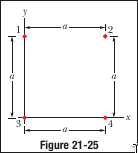
\includegraphics[scale=0.75]{image-4.png}
\end{figure}

\subsection*{Solution}
\textbf{Part a:} From the symmetry we just need to find the $Q/q$ such that 
\[
    F_{41,y} + F_{31} = 0
\]
which we can find by

\begin{align*}
    F_{41,y} &= k \frac{Q^2}{\left(\sqrt{2a^2}\right)^2} \sin\left(\frac{\pi}{4}\right)\\
    &= k \frac{Q^2}{2a^2} \cdot \frac{1}{\sqrt{2}}
\end{align*}
and

\begin{align*}
    F_{31} &= k \frac{Qq}{a^2}
\end{align*}
then

\begin{align*}
    k \frac{Q^2}{2a^2\sqrt{2}} + k \frac{Qq}{a^2} &= 0 \\
    k \frac{Q^2}{2a^2\sqrt{2}} &= - k \frac{Qq}{a^2} \\
    \frac{Q^2}{2\sqrt{2}} &= - Qq \\
    \frac{Q}{q} &= \boxed{- 2 \sqrt{2}}
\end{align*}
\textbf{Part b:} No, there is no value of $q$ that would result in each of the net forces being zero because of the mirror symmetry of the configuration. 
Meaning that $q/Q = -2\sqrt{2}$ if the net force on particle 3 is zero and it cannot be simultaneosly true that $q/Q = -2\sqrt{2} \wedge Q/q = -2\sqrt{2}$.

\section*{21-3 Problem 11}
In Fig. 21-25, the particles have charges $q1 = -q2 = 100$ nC and $q3 = -q4 = 200$ nC, and distance $a = 5.0$ cm. 
What are the (a) $x$ and (b) $y$ components of the net electrostatic force on particle 3?


\end{document}
